% Options for packages loaded elsewhere
% Options for packages loaded elsewhere
\PassOptionsToPackage{unicode}{hyperref}
\PassOptionsToPackage{hyphens}{url}
\PassOptionsToPackage{dvipsnames,svgnames,x11names}{xcolor}
%
\documentclass[
  spanish,
  11pt,
  a4paper,
  DIV=11,
  numbers=noendperiod]{scrartcl}
\usepackage{xcolor}
\usepackage[margin=2.5cm]{geometry}
\usepackage{amsmath,amssymb}
\setcounter{secnumdepth}{5}
\usepackage{iftex}
\ifPDFTeX
  \usepackage[T1]{fontenc}
  \usepackage[utf8]{inputenc}
  \usepackage{textcomp} % provide euro and other symbols
\else % if luatex or xetex
  \usepackage{unicode-math} % this also loads fontspec
  \defaultfontfeatures{Scale=MatchLowercase}
  \defaultfontfeatures[\rmfamily]{Ligatures=TeX,Scale=1}
\fi
\usepackage{lmodern}
\ifPDFTeX\else
  % xetex/luatex font selection
  \setmainfont[]{Times New Roman}
\fi
% Use upquote if available, for straight quotes in verbatim environments
\IfFileExists{upquote.sty}{\usepackage{upquote}}{}
\IfFileExists{microtype.sty}{% use microtype if available
  \usepackage[]{microtype}
  \UseMicrotypeSet[protrusion]{basicmath} % disable protrusion for tt fonts
}{}
\makeatletter
\@ifundefined{KOMAClassName}{% if non-KOMA class
  \IfFileExists{parskip.sty}{%
    \usepackage{parskip}
  }{% else
    \setlength{\parindent}{0pt}
    \setlength{\parskip}{6pt plus 2pt minus 1pt}}
}{% if KOMA class
  \KOMAoptions{parskip=half}}
\makeatother
% Make \paragraph and \subparagraph free-standing
\makeatletter
\ifx\paragraph\undefined\else
  \let\oldparagraph\paragraph
  \renewcommand{\paragraph}{
    \@ifstar
      \xxxParagraphStar
      \xxxParagraphNoStar
  }
  \newcommand{\xxxParagraphStar}[1]{\oldparagraph*{#1}\mbox{}}
  \newcommand{\xxxParagraphNoStar}[1]{\oldparagraph{#1}\mbox{}}
\fi
\ifx\subparagraph\undefined\else
  \let\oldsubparagraph\subparagraph
  \renewcommand{\subparagraph}{
    \@ifstar
      \xxxSubParagraphStar
      \xxxSubParagraphNoStar
  }
  \newcommand{\xxxSubParagraphStar}[1]{\oldsubparagraph*{#1}\mbox{}}
  \newcommand{\xxxSubParagraphNoStar}[1]{\oldsubparagraph{#1}\mbox{}}
\fi
\makeatother

\usepackage{color}
\usepackage{fancyvrb}
\newcommand{\VerbBar}{|}
\newcommand{\VERB}{\Verb[commandchars=\\\{\}]}
\DefineVerbatimEnvironment{Highlighting}{Verbatim}{commandchars=\\\{\}}
% Add ',fontsize=\small' for more characters per line
\usepackage{framed}
\definecolor{shadecolor}{RGB}{241,243,245}
\newenvironment{Shaded}{\begin{snugshade}}{\end{snugshade}}
\newcommand{\AlertTok}[1]{\textcolor[rgb]{0.68,0.00,0.00}{#1}}
\newcommand{\AnnotationTok}[1]{\textcolor[rgb]{0.37,0.37,0.37}{#1}}
\newcommand{\AttributeTok}[1]{\textcolor[rgb]{0.40,0.45,0.13}{#1}}
\newcommand{\BaseNTok}[1]{\textcolor[rgb]{0.68,0.00,0.00}{#1}}
\newcommand{\BuiltInTok}[1]{\textcolor[rgb]{0.00,0.23,0.31}{#1}}
\newcommand{\CharTok}[1]{\textcolor[rgb]{0.13,0.47,0.30}{#1}}
\newcommand{\CommentTok}[1]{\textcolor[rgb]{0.37,0.37,0.37}{#1}}
\newcommand{\CommentVarTok}[1]{\textcolor[rgb]{0.37,0.37,0.37}{\textit{#1}}}
\newcommand{\ConstantTok}[1]{\textcolor[rgb]{0.56,0.35,0.01}{#1}}
\newcommand{\ControlFlowTok}[1]{\textcolor[rgb]{0.00,0.23,0.31}{\textbf{#1}}}
\newcommand{\DataTypeTok}[1]{\textcolor[rgb]{0.68,0.00,0.00}{#1}}
\newcommand{\DecValTok}[1]{\textcolor[rgb]{0.68,0.00,0.00}{#1}}
\newcommand{\DocumentationTok}[1]{\textcolor[rgb]{0.37,0.37,0.37}{\textit{#1}}}
\newcommand{\ErrorTok}[1]{\textcolor[rgb]{0.68,0.00,0.00}{#1}}
\newcommand{\ExtensionTok}[1]{\textcolor[rgb]{0.00,0.23,0.31}{#1}}
\newcommand{\FloatTok}[1]{\textcolor[rgb]{0.68,0.00,0.00}{#1}}
\newcommand{\FunctionTok}[1]{\textcolor[rgb]{0.28,0.35,0.67}{#1}}
\newcommand{\ImportTok}[1]{\textcolor[rgb]{0.00,0.46,0.62}{#1}}
\newcommand{\InformationTok}[1]{\textcolor[rgb]{0.37,0.37,0.37}{#1}}
\newcommand{\KeywordTok}[1]{\textcolor[rgb]{0.00,0.23,0.31}{\textbf{#1}}}
\newcommand{\NormalTok}[1]{\textcolor[rgb]{0.00,0.23,0.31}{#1}}
\newcommand{\OperatorTok}[1]{\textcolor[rgb]{0.37,0.37,0.37}{#1}}
\newcommand{\OtherTok}[1]{\textcolor[rgb]{0.00,0.23,0.31}{#1}}
\newcommand{\PreprocessorTok}[1]{\textcolor[rgb]{0.68,0.00,0.00}{#1}}
\newcommand{\RegionMarkerTok}[1]{\textcolor[rgb]{0.00,0.23,0.31}{#1}}
\newcommand{\SpecialCharTok}[1]{\textcolor[rgb]{0.37,0.37,0.37}{#1}}
\newcommand{\SpecialStringTok}[1]{\textcolor[rgb]{0.13,0.47,0.30}{#1}}
\newcommand{\StringTok}[1]{\textcolor[rgb]{0.13,0.47,0.30}{#1}}
\newcommand{\VariableTok}[1]{\textcolor[rgb]{0.07,0.07,0.07}{#1}}
\newcommand{\VerbatimStringTok}[1]{\textcolor[rgb]{0.13,0.47,0.30}{#1}}
\newcommand{\WarningTok}[1]{\textcolor[rgb]{0.37,0.37,0.37}{\textit{#1}}}

\usepackage{longtable,booktabs,array}
\usepackage{calc} % for calculating minipage widths
% Correct order of tables after \paragraph or \subparagraph
\usepackage{etoolbox}
\makeatletter
\patchcmd\longtable{\par}{\if@noskipsec\mbox{}\fi\par}{}{}
\makeatother
% Allow footnotes in longtable head/foot
\IfFileExists{footnotehyper.sty}{\usepackage{footnotehyper}}{\usepackage{footnote}}
\makesavenoteenv{longtable}
\usepackage{graphicx}
\makeatletter
\newsavebox\pandoc@box
\newcommand*\pandocbounded[1]{% scales image to fit in text height/width
  \sbox\pandoc@box{#1}%
  \Gscale@div\@tempa{\textheight}{\dimexpr\ht\pandoc@box+\dp\pandoc@box\relax}%
  \Gscale@div\@tempb{\linewidth}{\wd\pandoc@box}%
  \ifdim\@tempb\p@<\@tempa\p@\let\@tempa\@tempb\fi% select the smaller of both
  \ifdim\@tempa\p@<\p@\scalebox{\@tempa}{\usebox\pandoc@box}%
  \else\usebox{\pandoc@box}%
  \fi%
}
% Set default figure placement to htbp
\def\fps@figure{htbp}
\makeatother



\ifLuaTeX
\usepackage[bidi=basic]{babel}
\else
\usepackage[bidi=default]{babel}
\fi
\ifPDFTeX
\else
\babelfont{rm}[]{Times New Roman}
\fi
% get rid of language-specific shorthands (see #6817):
\let\LanguageShortHands\languageshorthands
\def\languageshorthands#1{}


\setlength{\emergencystretch}{3em} % prevent overfull lines

\providecommand{\tightlist}{%
  \setlength{\itemsep}{0pt}\setlength{\parskip}{0pt}}



 


\KOMAoption{captions}{tableheading}
\makeatletter
\@ifpackageloaded{caption}{}{\usepackage{caption}}
\AtBeginDocument{%
\ifdefined\contentsname
  \renewcommand*\contentsname{Tabla de contenidos}
\else
  \newcommand\contentsname{Tabla de contenidos}
\fi
\ifdefined\listfigurename
  \renewcommand*\listfigurename{Listado de Figuras}
\else
  \newcommand\listfigurename{Listado de Figuras}
\fi
\ifdefined\listtablename
  \renewcommand*\listtablename{Listado de Tablas}
\else
  \newcommand\listtablename{Listado de Tablas}
\fi
\ifdefined\figurename
  \renewcommand*\figurename{Figura}
\else
  \newcommand\figurename{Figura}
\fi
\ifdefined\tablename
  \renewcommand*\tablename{Tabla}
\else
  \newcommand\tablename{Tabla}
\fi
}
\@ifpackageloaded{float}{}{\usepackage{float}}
\floatstyle{ruled}
\@ifundefined{c@chapter}{\newfloat{codelisting}{h}{lop}}{\newfloat{codelisting}{h}{lop}[chapter]}
\floatname{codelisting}{Listado}
\newcommand*\listoflistings{\listof{codelisting}{Listado de Listados}}
\makeatother
\makeatletter
\makeatother
\makeatletter
\@ifpackageloaded{caption}{}{\usepackage{caption}}
\@ifpackageloaded{subcaption}{}{\usepackage{subcaption}}
\makeatother
\usepackage{bookmark}
\IfFileExists{xurl.sty}{\usepackage{xurl}}{} % add URL line breaks if available
\urlstyle{same}
\hypersetup{
  pdftitle={Prueba de hipótesis},
  pdfauthor={Santos G},
  pdflang={es},
  colorlinks=true,
  linkcolor={blue},
  filecolor={Maroon},
  citecolor={Blue},
  urlcolor={Blue},
  pdfcreator={LaTeX via pandoc}}


\title{Prueba de hipótesis}
\author{Santos G}
\date{}
\begin{document}
\maketitle

\renewcommand*\contentsname{Tabla de contenidos}
{
\hypersetup{linkcolor=}
\setcounter{tocdepth}{2}
\tableofcontents
}

\section{Contexto del proyecto}\label{contexto-del-proyecto}

En este análisis trabajaremos con el dataset \texttt{palmerpenguins},
que contiene información morfométrica de tres especies (\emph{Adelie,
Chinstrap y Gentoo}). Previamente, los datos fueron limpiados y
verificados, de modo que ahora podemos avanzar hacia las pruebas
estadísticas que comparan medias entre grupos.

\textbf{Pregunta de investigación:} ¿Existen diferencias significativas
en el largo del pico (\emph{bill\_length\_mm}) entre las tres especies
de pingüinos?

\section{Carga de líbrerías y
datos}\label{carga-de-luxedbreruxedas-y-datos}

\begin{Shaded}
\begin{Highlighting}[numbers=left,,]
\FunctionTok{library}\NormalTok{(tidyverse)   }\CommentTok{\# dplyr, ggplot2, tidyr: manipulación de datos y gráficos}
\FunctionTok{library}\NormalTok{(janitor)     }\CommentTok{\# clean\_names(): estandarizar nombres de variables}
\FunctionTok{library}\NormalTok{(palmerpenguins) }\CommentTok{\# dataset de ejemplo (penguins)}
\FunctionTok{library}\NormalTok{(car)         }\CommentTok{\# leveneTest(): prueba de homogeneidad de varianzas}
\FunctionTok{library}\NormalTok{(rstatix)     }\CommentTok{\# funciones rápidas para ANOVA, Kruskal–Wallis, post{-}hoc}
\FunctionTok{library}\NormalTok{(ggpubr)      }\CommentTok{\# visualización de resultados estadísticos}

\NormalTok{df\_raw }\OtherTok{\textless{}{-}}\NormalTok{ penguins }\SpecialCharTok{\%\textgreater{}\%} \FunctionTok{as\_tibble}\NormalTok{() }\CommentTok{\# guardo raw para auditoría}
\NormalTok{df }\OtherTok{\textless{}{-}}\NormalTok{ df\_raw }\SpecialCharTok{\%\textgreater{}\%} \FunctionTok{clean\_names}\NormalTok{()}
\end{Highlighting}
\end{Shaded}

\section{Verificación de supuestos}\label{verificaciuxf3n-de-supuestos}

\begin{Shaded}
\begin{Highlighting}[numbers=left,,]
\NormalTok{modelo }\OtherTok{\textless{}{-}} \FunctionTok{aov}\NormalTok{(bill\_length\_mm }\SpecialCharTok{\textasciitilde{}}\NormalTok{ species, }\AttributeTok{data =}\NormalTok{ df)                                  }

\CommentTok{\# Normalidad de residuos}
\NormalTok{Normalidad }\OtherTok{\textless{}{-}} \FunctionTok{shapiro.test}\NormalTok{(}\FunctionTok{residuals}\NormalTok{(modelo))}

\CommentTok{\# Homogeneidad de varianzas (Levene)}
\NormalTok{Homogeneidad }\OtherTok{\textless{}{-}} \FunctionTok{leveneTest}\NormalTok{(bill\_length\_mm }\SpecialCharTok{\textasciitilde{}}\NormalTok{ species, }\AttributeTok{data =}\NormalTok{ df)}

\CommentTok{\# Tablas}
\NormalTok{knitr}\SpecialCharTok{::}\FunctionTok{kable}\NormalTok{(}
\NormalTok{  broom}\SpecialCharTok{::}\FunctionTok{tidy}\NormalTok{(Normalidad),}
  \AttributeTok{caption =} \StringTok{"Test de normalidad de residuos (Shapiro{-}Wilk)"}
\NormalTok{)}
\end{Highlighting}
\end{Shaded}

\begin{longtable}[]{@{}rrl@{}}
\caption{Test de normalidad de residuos (Shapiro-Wilk)}\tabularnewline
\toprule\noalign{}
statistic & p.value & method \\
\midrule\noalign{}
\endfirsthead
\toprule\noalign{}
statistic & p.value & method \\
\midrule\noalign{}
\endhead
\bottomrule\noalign{}
\endlastfoot
0.9890313 & 0.0113053 & Shapiro-Wilk normality test \\
\end{longtable}

\begin{Shaded}
\begin{Highlighting}[numbers=left,,]
\NormalTok{knitr}\SpecialCharTok{::}\FunctionTok{kable}\NormalTok{(}
\NormalTok{  broom}\SpecialCharTok{::}\FunctionTok{tidy}\NormalTok{(Homogeneidad),}
  \AttributeTok{caption =} \StringTok{"Test de homogeneidad de varianzas (Levene)"}
\NormalTok{)}
\end{Highlighting}
\end{Shaded}

\begin{longtable}[]{@{}rrrr@{}}
\caption{Test de homogeneidad de varianzas (Levene)}\tabularnewline
\toprule\noalign{}
statistic & p.value & df & df.residual \\
\midrule\noalign{}
\endfirsthead
\toprule\noalign{}
statistic & p.value & df & df.residual \\
\midrule\noalign{}
\endhead
\bottomrule\noalign{}
\endlastfoot
2.242456 & 0.1077705 & 2 & 339 \\
\end{longtable}

En la \textbf{Tabla 1} se presentan los resultados del test
Shapiro--Wilk (W = 0.989, p = 0.0113 ) el valor p es menor a 0.05; por
lo tanto, se rechaza la normalidad de los residuos. En cuanto a la
homogeneidad de varianzas, en la \textbf{Tabla 2} se reflejan los
resultados del test de Levene (F = 2.242, p = 0.108 ) arrojó un valor p
mayor a 0.05, lo que indica que no se rechaza este supuesto, es decir
las varianzas entre grupos pueden considerarse similares.

En consecuencia, dado que el supuesto de normalidad no se cumple, aunque
sí el de homogeneidad de varianzas, la opción más segura y robusta es
realizar Kruskal--Wallis (prueba no paramétrica).

\section{Ejeccución del Kruskal-Wallis
global}\label{ejeccuciuxf3n-del-kruskal-wallis-global}

\begin{Shaded}
\begin{Highlighting}[numbers=left,,]
\CommentTok{\# Kruskal{-}Wallis (global)}
\NormalTok{kruskal\_res }\OtherTok{\textless{}{-}}\NormalTok{ df }\SpecialCharTok{\%\textgreater{}\%} \FunctionTok{kruskal\_test}\NormalTok{(bill\_length\_mm }\SpecialCharTok{\textasciitilde{}}\NormalTok{ species)}

\CommentTok{\# Formatear p{-}value como p \textless{} 0.001 si es muy pequeño}
\NormalTok{kruskal\_res }\OtherTok{\textless{}{-}}\NormalTok{ kruskal\_res }\SpecialCharTok{\%\textgreater{}\%}
  \FunctionTok{mutate}\NormalTok{(}\AttributeTok{p =} \FunctionTok{ifelse}\NormalTok{(p }\SpecialCharTok{\textless{}} \FloatTok{0.001}\NormalTok{, }\StringTok{"\textless{} 0.001"}\NormalTok{, }\FunctionTok{round}\NormalTok{(p, }\DecValTok{3}\NormalTok{)))}

\NormalTok{knitr}\SpecialCharTok{::}\FunctionTok{kable}\NormalTok{(kruskal\_res, }\AttributeTok{caption =} \StringTok{"Prueba Kruskal{-}Wallis global"}\NormalTok{)}
\end{Highlighting}
\end{Shaded}

\begin{longtable}[]{@{}lrrrll@{}}
\caption{Prueba Kruskal-Wallis global}\tabularnewline
\toprule\noalign{}
.y. & n & statistic & df & p & method \\
\midrule\noalign{}
\endfirsthead
\toprule\noalign{}
.y. & n & statistic & df & p & method \\
\midrule\noalign{}
\endhead
\bottomrule\noalign{}
\endlastfoot
bill\_length\_mm & 342 & 244.1367 & 2 & \textless{} 0.001 &
Kruskal-Wallis \\
\end{longtable}

En la \textbf{Tabla 3} se presentan los resultados de la prueba de
Kruskal--Wallis: χ² = 244.14, gl = 2, p = \textless{} 0.001. El valor p
es mucho menor a 0.001, lo que indica diferencias altamente
significativas en el largo del pico entre las tres especies de
pingüinos.

\begin{Shaded}
\begin{Highlighting}[numbers=left,,]
\CommentTok{\# Tamaño de efecto (epsilon{-}squared)}
\NormalTok{Efe }\OtherTok{\textless{}{-}}\NormalTok{ df }\SpecialCharTok{\%\textgreater{}\%} \FunctionTok{kruskal\_effsize}\NormalTok{(bill\_length\_mm }\SpecialCharTok{\textasciitilde{}}\NormalTok{ species)}
\NormalTok{knitr}\SpecialCharTok{::}\FunctionTok{kable}\NormalTok{(Efe, }\AttributeTok{caption =} \StringTok{"Tamaño de efecto (epsilon{-}squared)"}\NormalTok{)}
\end{Highlighting}
\end{Shaded}

\begin{longtable}[]{@{}lrrll@{}}
\caption{Tamaño de efecto (epsilon-squared)}\tabularnewline
\toprule\noalign{}
.y. & n & effsize & method & magnitude \\
\midrule\noalign{}
\endfirsthead
\toprule\noalign{}
.y. & n & effsize & method & magnitude \\
\midrule\noalign{}
\endhead
\bottomrule\noalign{}
\endlastfoot
bill\_length\_mm & 342 & 0.7142676 & eta2{[}H{]} & large \\
\end{longtable}

En la \textbf{Tabla 4} se muestra el tamaño de efecto (ε²): 0.7142676.
Este resultado confirma que la magnitud de estas diferencias es muy
grande: la variable ``especie'' explica aproximadamente el 71\% de la
variación en el largo del pico. Esto significa que el largo del pico no
varía al azar, sino que está fuertemente determinado por la especie.

\section{Comparaciones post-hoc (Dunn, corrección
Bonferroni)}\label{comparaciones-post-hoc-dunn-correcciuxf3n-bonferroni}

\begin{Shaded}
\begin{Highlighting}[numbers=left,,]
\CommentTok{\# Dunn test con corrección Bonferroni}
\NormalTok{dunn\_res }\OtherTok{\textless{}{-}}\NormalTok{ df }\SpecialCharTok{\%\textgreater{}\%}
  \FunctionTok{dunn\_test}\NormalTok{(bill\_length\_mm }\SpecialCharTok{\textasciitilde{}}\NormalTok{ species, }\AttributeTok{p.adjust.method =} \StringTok{"bonferroni"}\NormalTok{) }\SpecialCharTok{\%\textgreater{}\%}
  \FunctionTok{mutate}\NormalTok{(}\AttributeTok{p =} \FunctionTok{ifelse}\NormalTok{(p }\SpecialCharTok{\textless{}} \FloatTok{0.001}\NormalTok{, }\StringTok{"\textless{} 0.001"}\NormalTok{, }\FunctionTok{round}\NormalTok{(p, }\DecValTok{3}\NormalTok{)),}
         \AttributeTok{p.adj =} \FunctionTok{ifelse}\NormalTok{(p.adj }\SpecialCharTok{\textless{}} \FloatTok{0.001}\NormalTok{, }\StringTok{"\textless{} 0.001"}\NormalTok{, }\FunctionTok{round}\NormalTok{(p.adj, }\DecValTok{3}\NormalTok{)))}

\NormalTok{knitr}\SpecialCharTok{::}\FunctionTok{kable}\NormalTok{(dunn\_res, }\AttributeTok{caption =} \StringTok{"Comparaciones post{-}hoc (Dunn, Bonferroni)"}\NormalTok{)}
\end{Highlighting}
\end{Shaded}

\begin{longtable}[]{@{}
  >{\raggedright\arraybackslash}p{(\linewidth - 16\tabcolsep) * \real{0.1829}}
  >{\raggedright\arraybackslash}p{(\linewidth - 16\tabcolsep) * \real{0.1220}}
  >{\raggedright\arraybackslash}p{(\linewidth - 16\tabcolsep) * \real{0.1220}}
  >{\raggedleft\arraybackslash}p{(\linewidth - 16\tabcolsep) * \real{0.0488}}
  >{\raggedleft\arraybackslash}p{(\linewidth - 16\tabcolsep) * \real{0.0488}}
  >{\raggedleft\arraybackslash}p{(\linewidth - 16\tabcolsep) * \real{0.1220}}
  >{\raggedright\arraybackslash}p{(\linewidth - 16\tabcolsep) * \real{0.0976}}
  >{\raggedright\arraybackslash}p{(\linewidth - 16\tabcolsep) * \real{0.0976}}
  >{\raggedright\arraybackslash}p{(\linewidth - 16\tabcolsep) * \real{0.1585}}@{}}
\caption{Comparaciones post-hoc (Dunn, Bonferroni)}\tabularnewline
\toprule\noalign{}
\begin{minipage}[b]{\linewidth}\raggedright
.y.
\end{minipage} & \begin{minipage}[b]{\linewidth}\raggedright
group1
\end{minipage} & \begin{minipage}[b]{\linewidth}\raggedright
group2
\end{minipage} & \begin{minipage}[b]{\linewidth}\raggedleft
n1
\end{minipage} & \begin{minipage}[b]{\linewidth}\raggedleft
n2
\end{minipage} & \begin{minipage}[b]{\linewidth}\raggedleft
statistic
\end{minipage} & \begin{minipage}[b]{\linewidth}\raggedright
p
\end{minipage} & \begin{minipage}[b]{\linewidth}\raggedright
p.adj
\end{minipage} & \begin{minipage}[b]{\linewidth}\raggedright
p.adj.signif
\end{minipage} \\
\midrule\noalign{}
\endfirsthead
\toprule\noalign{}
\begin{minipage}[b]{\linewidth}\raggedright
.y.
\end{minipage} & \begin{minipage}[b]{\linewidth}\raggedright
group1
\end{minipage} & \begin{minipage}[b]{\linewidth}\raggedright
group2
\end{minipage} & \begin{minipage}[b]{\linewidth}\raggedleft
n1
\end{minipage} & \begin{minipage}[b]{\linewidth}\raggedleft
n2
\end{minipage} & \begin{minipage}[b]{\linewidth}\raggedleft
statistic
\end{minipage} & \begin{minipage}[b]{\linewidth}\raggedright
p
\end{minipage} & \begin{minipage}[b]{\linewidth}\raggedright
p.adj
\end{minipage} & \begin{minipage}[b]{\linewidth}\raggedright
p.adj.signif
\end{minipage} \\
\midrule\noalign{}
\endhead
\bottomrule\noalign{}
\endlastfoot
bill\_length\_mm & Adelie & Chinstrap & 151 & 68 & 12.753511 &
\textless{} 0.001 & \textless{} 0.001 & **** \\
bill\_length\_mm & Adelie & Gentoo & 151 & 123 & 13.135630 & \textless{}
0.001 & \textless{} 0.001 & **** \\
bill\_length\_mm & Chinstrap & Gentoo & 68 & 123 & -1.767498 & 0.077 &
0.231 & ns \\
\end{longtable}

En la \textbf{Tabla 5} se presentan las comparaciones por pares (Dunn,
Bonferroni):

\begin{itemize}
\item
  \emph{Adelie} vs \emph{Chinstrap}: p.adj = \textless{} 0.001 →
  significativo (****).
\item
  \emph{Adelie} vs \emph{Gentoo}: p.adj = \textless{} 0.001 →
  significativo (****).
\item
  \emph{Chinstrap} vs \emph{Gentoo}: p.adj = 0.231 → no significativo
  (ns).
\end{itemize}

Las comparaciones muestran que el largo del pico en \emph{Adelie}
difiere significativamente tanto de \emph{Chinstrap} como de
\emph{Gentoo}. Mientras que entre \emph{Chinstrap} y \emph{Gentoo} no se
detectan diferencias estadísticamente significativas en el largo del
pico. Esto sugiere que la dieta de \emph{Adelie} es distinta a la de las
otras especies. Mientras que entre \emph{Gentoo} y \emph{Chinstrap},
podrían compartir parcialmente los mismos recursos tróficos. En
conjunto, la prueba confirma una clara segregación de \emph{Adelie}
respecto a las otras especies, lo que reduce la competencia y favorece
la coexistencia de las tres especies en el ecosistema antártico.

\begin{Shaded}
\begin{Highlighting}[numbers=left,,]
\CommentTok{\# Añadir posiciones y columnas útiles para gráficas}
\NormalTok{dunn\_res }\OtherTok{\textless{}{-}}\NormalTok{ dunn\_res }\SpecialCharTok{\%\textgreater{}\%} \FunctionTok{add\_xy\_position}\NormalTok{(}\AttributeTok{x =} \StringTok{"species"}\NormalTok{)}

\CommentTok{\# Calcula un y{-}position razonable para las etiquetas}
\NormalTok{y\_max }\OtherTok{\textless{}{-}} \FunctionTok{max}\NormalTok{(df}\SpecialCharTok{$}\NormalTok{bill\_length\_mm, }\AttributeTok{na.rm =} \ConstantTok{TRUE}\NormalTok{)}
\NormalTok{dunn\_res }\OtherTok{\textless{}{-}}\NormalTok{ dunn\_res }\SpecialCharTok{\%\textgreater{}\%} \FunctionTok{mutate}\NormalTok{(}\AttributeTok{y.position =}\NormalTok{ y\_max }\SpecialCharTok{+} \FunctionTok{seq}\NormalTok{(}\FloatTok{0.5}\NormalTok{, }\AttributeTok{by =} \FloatTok{0.5}\NormalTok{, }
  \AttributeTok{length.out =} \FunctionTok{nrow}\NormalTok{(dunn\_res)))}

\NormalTok{p }\OtherTok{\textless{}{-}} \FunctionTok{ggplot}\NormalTok{(df, }\FunctionTok{aes}\NormalTok{(}\AttributeTok{x =}\NormalTok{ species, }\AttributeTok{y =}\NormalTok{ bill\_length\_mm, }\AttributeTok{fill =}\NormalTok{ species)) }\SpecialCharTok{+}
  \FunctionTok{geom\_boxplot}\NormalTok{(}\AttributeTok{alpha =} \FloatTok{0.7}\NormalTok{) }\SpecialCharTok{+}
  \FunctionTok{geom\_jitter}\NormalTok{(}\AttributeTok{width =} \FloatTok{0.15}\NormalTok{, }\AttributeTok{alpha =} \FloatTok{0.5}\NormalTok{, }\AttributeTok{size =} \DecValTok{1}\NormalTok{) }\SpecialCharTok{+}
  \FunctionTok{theme\_minimal}\NormalTok{() }\SpecialCharTok{+}
  \FunctionTok{theme}\NormalTok{(}\AttributeTok{legend.position =} \StringTok{"none"}\NormalTok{) }\SpecialCharTok{+}
  \FunctionTok{labs}\NormalTok{(}\AttributeTok{x =} \StringTok{"Especie"}\NormalTok{, }\AttributeTok{y =} \StringTok{"Largo del pico (mm)"}\NormalTok{,}
       \AttributeTok{title =} \StringTok{"Comparación del largo del pico entre especies"}\NormalTok{)}

\CommentTok{\# Añadir anotaciones de p ajustadas}
\NormalTok{p }\SpecialCharTok{+}\NormalTok{ ggpubr}\SpecialCharTok{::}\FunctionTok{stat\_pvalue\_manual}\NormalTok{(dunn\_res, }\AttributeTok{label =} \StringTok{"p.adj.signif"}\NormalTok{, }
    \AttributeTok{tip.length =} \FloatTok{0.01}\NormalTok{)}
\end{Highlighting}
\end{Shaded}

\begin{figure}[H]

{\centering \pandocbounded{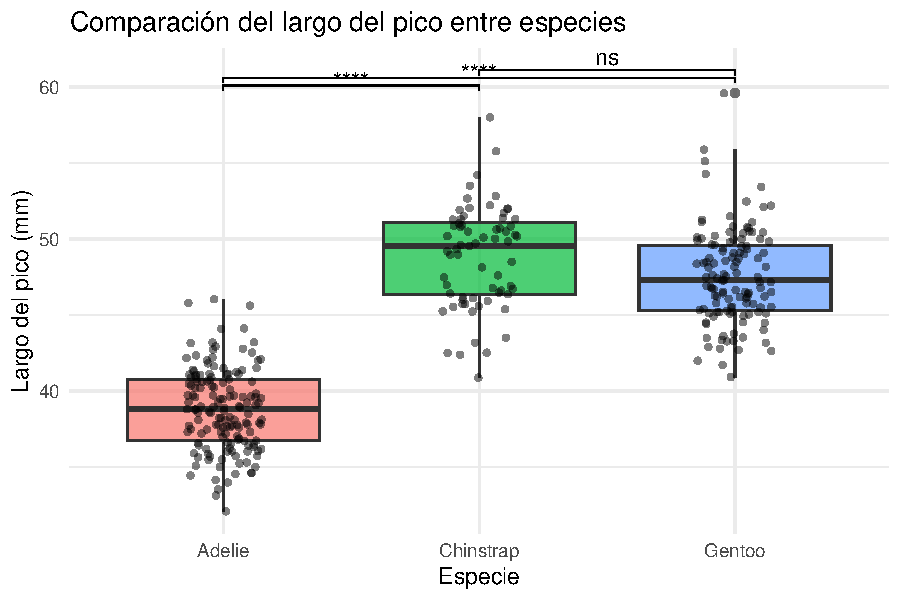
\includegraphics[keepaspectratio]{Prueba-de-hipotesis_files/figure-pdf/boxplot_kruskal-1.pdf}}

}

\caption{Boxplot de bill\_length\_mm por especie con comparaciones
post-hoc (Dunn).}

\end{figure}%

La \textbf{Figura 1} muestra la distribución del largo del pico en las
tres especies de pingüinos (\emph{Adelie}, \emph{Chinstrap} y
\emph{Gentoo}). Se observa que los \emph{Adelie} presentan valores
menores y más concentrados (mediana cercana a 38--40 mm), mientras que
los \emph{Chinstrap} tienen los picos más largos (mediana en torno a
48--50 mm). Los \emph{Gentoo} ocupan una posición intermedia, con
valores cercanos a 46--48 mm y mayor variabilidad en comparación con
\emph{Adelie}.

Las comparaciones post-hoc de Dunn con corrección de Bonferroni
evidencian diferencias altamente significativas en \emph{Adelie vs
Chinstrap} (****) y \emph{Adelie vs Gentoo} (****\emph{).} Por el
contrario, no se encontraron diferencias significativas entre
\emph{Chinstrap} vs \emph{Gentoo} (ns).

\section{Conclusiones
Kruskall-Wallis}\label{conclusiones-kruskall-wallis}

\begin{itemize}
\item
  El análisis estadístico mediante Kruskal--Wallis confirmó diferencias
  significativas en la distribución del largo del pico entre especies de
  pingüinos (χ² = 244.1, p \textless{} 0.001), con un tamaño de efecto
  muy grande (ε² = 0.71). Esto indica que la especie explica una
  proporción sustancial de la variabilidad observada en la morfología
  del pico.
\item
  Las pruebas post-hoc mostraron que los \emph{Adelie} difieren
  significativamente de \emph{Chinstrap} y \emph{Gentoo}, mientras que
  estas dos últimas no presentan diferencias estadísticamente
  significativas entre sí.
\item
  Desde una perspectiva ecológica, los resultados sugieren que
  \emph{Adelie} ocupa un nicho trófico diferenciado, asociado al consumo
  de krill y pequeños invertebrados, lo que reduce la competencia
  directa con las otras especies. En cambio, \emph{Gentoo} y
  \emph{Chinstrap}, al presentar longitudes de pico más similares,
  podrían solaparse en el aprovechamiento de presas de mayor tamaño
  (peces e invertebrados grandes).
\item
  En conjunto, los hallazgos respaldan la hipótesis de una segregación
  morfológica y trófica que favorece la coexistencia de las tres
  especies en el ecosistema antártico.
\end{itemize}

\section{Anova con transformación
logarítmica}\label{anova-con-transformaciuxf3n-logaruxedtmica}

\begin{Shaded}
\begin{Highlighting}[numbers=left,,]
\NormalTok{df }\OtherTok{\textless{}{-}}\NormalTok{ df }\SpecialCharTok{\%\textgreater{}\%}
  \FunctionTok{mutate}\NormalTok{(}\AttributeTok{log\_bill\_length =} \FunctionTok{log}\NormalTok{(bill\_length\_mm))}
\NormalTok{modelo\_log }\OtherTok{\textless{}{-}} \FunctionTok{aov}\NormalTok{(log\_bill\_length }\SpecialCharTok{\textasciitilde{}}\NormalTok{ species, }\AttributeTok{data =}\NormalTok{ df)}

\CommentTok{\# Supuestos}
\NormalTok{shapiro\_res }\OtherTok{\textless{}{-}} \FunctionTok{shapiro.test}\NormalTok{(}\FunctionTok{residuals}\NormalTok{(modelo\_log))}
\NormalTok{levene\_res  }\OtherTok{\textless{}{-}} \FunctionTok{leveneTest}\NormalTok{(log\_bill\_length }\SpecialCharTok{\textasciitilde{}}\NormalTok{ species, }\AttributeTok{data =}\NormalTok{ df)}

\CommentTok{\# Tablas}
\NormalTok{knitr}\SpecialCharTok{::}\FunctionTok{kable}\NormalTok{(}
\NormalTok{  broom}\SpecialCharTok{::}\FunctionTok{tidy}\NormalTok{(shapiro\_res),}
  \AttributeTok{caption =} \StringTok{"Test de normalidad de residuos (Shapiro{-}Wilk)"}
\NormalTok{)}
\end{Highlighting}
\end{Shaded}

\begin{longtable}[]{@{}rrl@{}}
\caption{Test de normalidad de residuos (Shapiro-Wilk)}\tabularnewline
\toprule\noalign{}
statistic & p.value & method \\
\midrule\noalign{}
\endfirsthead
\toprule\noalign{}
statistic & p.value & method \\
\midrule\noalign{}
\endhead
\bottomrule\noalign{}
\endlastfoot
0.9945676 & 0.2675526 & Shapiro-Wilk normality test \\
\end{longtable}

\begin{Shaded}
\begin{Highlighting}[numbers=left,,]
\NormalTok{knitr}\SpecialCharTok{::}\FunctionTok{kable}\NormalTok{(}
\NormalTok{  broom}\SpecialCharTok{::}\FunctionTok{tidy}\NormalTok{(levene\_res),}
  \AttributeTok{caption =} \StringTok{"Test de homogeneidad de varianzas (Levene)"}
\NormalTok{)}
\end{Highlighting}
\end{Shaded}

\begin{longtable}[]{@{}rrrr@{}}
\caption{Test de homogeneidad de varianzas (Levene)}\tabularnewline
\toprule\noalign{}
statistic & p.value & df & df.residual \\
\midrule\noalign{}
\endfirsthead
\toprule\noalign{}
statistic & p.value & df & df.residual \\
\midrule\noalign{}
\endhead
\bottomrule\noalign{}
\endlastfoot
0.5610386 & 0.571145 & 2 & 339 \\
\end{longtable}

En la \textbf{Tabla 6} se presentan los resultados del test
Shapiro--Wilk (W = 0.995, p = 0.268 ) el valor p es mayor a 0.05; por lo
tanto, no se rechaza la normalidad de los residuos. En cuanto a la
homogeneidad de varianzas, en la \textbf{Tabla 7} se reflejan los
resultados del test de Levene (F = 0.561, p = 0.571 ) arrojó un valor p
mayor a 0.05, lo que indica que no se rechaza este supuesto, es decir
las varianzas entre grupos pueden considerarse similares.

\begin{Shaded}
\begin{Highlighting}[numbers=left,,]
\CommentTok{\# Guardar en tidy para columnas limpias}
\NormalTok{anova\_res }\OtherTok{\textless{}{-}}\NormalTok{ broom}\SpecialCharTok{::}\FunctionTok{tidy}\NormalTok{(modelo\_log) }\SpecialCharTok{\%\textgreater{}\%}
  \FunctionTok{mutate}\NormalTok{(}\AttributeTok{p.value =} \FunctionTok{case\_when}\NormalTok{(}
\NormalTok{    p.value }\SpecialCharTok{\textless{}} \FloatTok{0.001} \SpecialCharTok{\textasciitilde{}} \StringTok{"\textless{} 0.001"}\NormalTok{,}
    \ConstantTok{TRUE} \SpecialCharTok{\textasciitilde{}} \FunctionTok{as.character}\NormalTok{(}\FunctionTok{round}\NormalTok{(p.value, }\DecValTok{3}\NormalTok{))}
\NormalTok{  ))}
\NormalTok{knitr}\SpecialCharTok{::}\FunctionTok{kable}\NormalTok{(}
\NormalTok{  anova\_res,}
  \AttributeTok{caption =} \StringTok{"Resultados de la prueba ANOVA (log{-}transformado)"}
\NormalTok{)}
\end{Highlighting}
\end{Shaded}

\begin{longtable}[]{@{}lrrrrl@{}}
\caption{Resultados de la prueba ANOVA
(log-transformado)}\tabularnewline
\toprule\noalign{}
term & df & sumsq & meansq & statistic & p.value \\
\midrule\noalign{}
\endfirsthead
\toprule\noalign{}
term & df & sumsq & meansq & statistic & p.value \\
\midrule\noalign{}
\endhead
\bottomrule\noalign{}
\endlastfoot
species & 2 & 3.846076 & 1.9230382 & 427.5831 & \textless{} 0.001 \\
Residuals & 339 & 1.524639 & 0.0044975 & NA & NA \\
\end{longtable}

En la \textbf{Tabla 8} se presentan los resultados de la prueba de ANOVA
(log-transformado): F = 427.6, gl = 2, p \textless{} 0.001. El valor p
es mucho menor a 0.001, lo que indica diferencias altamente
significativas en el largo del pico entre las tres especies de
pingüinos.

\section{Comparaciones post-hoc (Tukey
HSD)}\label{comparaciones-post-hoc-tukey-hsd}

\begin{Shaded}
\begin{Highlighting}[numbers=left,,]
\NormalTok{tukey\_res }\OtherTok{\textless{}{-}} \FunctionTok{TukeyHSD}\NormalTok{(modelo\_log)}

\NormalTok{tukey\_table }\OtherTok{\textless{}{-}}\NormalTok{ broom}\SpecialCharTok{::}\FunctionTok{tidy}\NormalTok{(tukey\_res) }\SpecialCharTok{\%\textgreater{}\%}
  \FunctionTok{mutate}\NormalTok{(}
    \AttributeTok{adj.p.value =} \FunctionTok{case\_when}\NormalTok{(}
\NormalTok{      adj.p.value }\SpecialCharTok{\textless{}} \FloatTok{0.001} \SpecialCharTok{\textasciitilde{}} \StringTok{"\textless{} 0.001"}\NormalTok{,}
      \ConstantTok{TRUE} \SpecialCharTok{\textasciitilde{}} \FunctionTok{as.character}\NormalTok{(}\FunctionTok{round}\NormalTok{(adj.p.value, }\DecValTok{3}\NormalTok{))}
\NormalTok{    ),}
    \AttributeTok{signif =} \FunctionTok{case\_when}\NormalTok{(}
\NormalTok{      adj.p.value }\SpecialCharTok{==} \StringTok{"\textless{} 0.001"} \SpecialCharTok{\textasciitilde{}} \StringTok{"***"}\NormalTok{,}
      \FunctionTok{as.numeric}\NormalTok{(adj.p.value) }\SpecialCharTok{\textless{}} \FloatTok{0.01}  \SpecialCharTok{\textasciitilde{}} \StringTok{"**"}\NormalTok{,}
      \FunctionTok{as.numeric}\NormalTok{(adj.p.value) }\SpecialCharTok{\textless{}} \FloatTok{0.05}  \SpecialCharTok{\textasciitilde{}} \StringTok{"*"}\NormalTok{,}
      \ConstantTok{TRUE} \SpecialCharTok{\textasciitilde{}} \StringTok{"ns"}
\NormalTok{    )}
\NormalTok{  )}

\NormalTok{knitr}\SpecialCharTok{::}\FunctionTok{kable}\NormalTok{(}
\NormalTok{  tukey\_table,}
  \AttributeTok{caption =} \StringTok{"Comparaciones post{-}hoc (Tukey HSD)"}
\NormalTok{)}
\end{Highlighting}
\end{Shaded}

\begin{longtable}[]{@{}
  >{\raggedright\arraybackslash}p{(\linewidth - 14\tabcolsep) * \real{0.0909}}
  >{\raggedright\arraybackslash}p{(\linewidth - 14\tabcolsep) * \real{0.1932}}
  >{\raggedleft\arraybackslash}p{(\linewidth - 14\tabcolsep) * \real{0.1250}}
  >{\raggedleft\arraybackslash}p{(\linewidth - 14\tabcolsep) * \real{0.1250}}
  >{\raggedleft\arraybackslash}p{(\linewidth - 14\tabcolsep) * \real{0.1250}}
  >{\raggedleft\arraybackslash}p{(\linewidth - 14\tabcolsep) * \real{0.1250}}
  >{\raggedright\arraybackslash}p{(\linewidth - 14\tabcolsep) * \real{0.1364}}
  >{\raggedright\arraybackslash}p{(\linewidth - 14\tabcolsep) * \real{0.0795}}@{}}
\caption{Comparaciones post-hoc (Tukey HSD)}\tabularnewline
\toprule\noalign{}
\begin{minipage}[b]{\linewidth}\raggedright
term
\end{minipage} & \begin{minipage}[b]{\linewidth}\raggedright
contrast
\end{minipage} & \begin{minipage}[b]{\linewidth}\raggedleft
null.value
\end{minipage} & \begin{minipage}[b]{\linewidth}\raggedleft
estimate
\end{minipage} & \begin{minipage}[b]{\linewidth}\raggedleft
conf.low
\end{minipage} & \begin{minipage}[b]{\linewidth}\raggedleft
conf.high
\end{minipage} & \begin{minipage}[b]{\linewidth}\raggedright
adj.p.value
\end{minipage} & \begin{minipage}[b]{\linewidth}\raggedright
signif
\end{minipage} \\
\midrule\noalign{}
\endfirsthead
\toprule\noalign{}
\begin{minipage}[b]{\linewidth}\raggedright
term
\end{minipage} & \begin{minipage}[b]{\linewidth}\raggedright
contrast
\end{minipage} & \begin{minipage}[b]{\linewidth}\raggedleft
null.value
\end{minipage} & \begin{minipage}[b]{\linewidth}\raggedleft
estimate
\end{minipage} & \begin{minipage}[b]{\linewidth}\raggedleft
conf.low
\end{minipage} & \begin{minipage}[b]{\linewidth}\raggedleft
conf.high
\end{minipage} & \begin{minipage}[b]{\linewidth}\raggedright
adj.p.value
\end{minipage} & \begin{minipage}[b]{\linewidth}\raggedright
signif
\end{minipage} \\
\midrule\noalign{}
\endhead
\bottomrule\noalign{}
\endlastfoot
species & Chinstrap-Adelie & 0 & 0.2302359 & 0.2071801 & 0.2532916 &
\textless{} 0.001 & *** \\
species & Gentoo-Adelie & 0 & 0.2029276 & 0.1837526 & 0.2221025 &
\textless{} 0.001 & *** \\
species & Gentoo-Chinstrap & 0 & -0.0273083 & -0.0511650 & -0.0034516 &
0.02 & * \\
\end{longtable}

En la \textbf{Tabla 9} se presentan los resultados de las comparaciones
por pares (Tukey HSD):

\begin{itemize}
\tightlist
\item
  \emph{Adelie vs Chinstrap:} p.adj = \textless{} 0.001 → diferencia
  altamente significativa (***).\\
\item
  \emph{Adelie vs Gentoo:} p.adj = \textless{} 0.001 → diferencia
  altamente significativa (***).\\
\item
  \emph{Chinstrap vs Gentoo:} p.adj = 0.02 → diferencia significativa,
  aunque de magnitud menor (*).
\end{itemize}

Los resultados muestran que el largo del pico en \emph{Adelie} difiere
de forma marcada respecto a \emph{Chinstrap} y \emph{Gentoo}. En
contraste, \emph{Chinstrap} y \emph{Gentoo} presentan una diferencia
estadísticamente significativa pero pequeña, lo que sugiere cierto
solapamiento ecológico entre ambas especies.

En conjunto, la prueba confirma una clara segregación de \emph{Adelie}
en términos de morfología y, por extensión, de dieta (más especializada
en krill e invertebrados pequeños). Por otro lado, \emph{Chinstrap} y
\emph{Gentoo} parecen compartir parcialmente los mismos recursos
tróficos, aunque mantienen diferencias detectables. Esto apoya la
hipótesis de que la diversificación morfológica reduce la competencia y
favorece la coexistencia de las tres especies en el ecosistema
antártico.

\section{Conclusiones Anova
(log-transformado)}\label{conclusiones-anova-log-transformado}

\begin{itemize}
\item
  El ANOVA con transformación logarítmica confirmó diferencias
  significativas en el largo del pico entre especies (F = 427.6, p
  \textless{} 0.001).
\item
  El post-hoc Tukey corroboró que \emph{Adelie} difiere de
  \emph{Chinstrap} y \emph{Gentoo}, y además detectó una diferencia
  débil pero significativa entre Chinstrap y Gentoo (p = 0.02).
\item
  Desde un punto de vista ecológico ambos enfoques concuerdan en que
  \emph{Adelie} presenta un nicho trófico diferenciado (picos más cortos
  y especializados en krill e invertebrados pequeños). Por su parte,
  \emph{Chinstrap} y \emph{Gentoo} muestran solapamiento parcial, aunque
  el ANOVA sugiere cierta divergencia morfológica que podría traducirse
  en un aprovechamiento diferenciado de los recursos.
\end{itemize}

Esto complementa los hallazgos del Kruskal--Wallis: mientras este último
no detectó diferencias entre \emph{Chinstrap} y \emph{Gentoo}, el ANOVA
más sensible identificó una separación sutil.




\end{document}
